\subsection{RQ3: weather robustness and resilient designs}
For policy or design $x$, let $J(x,\omega)$ be its simulated mean payoff under scenario $\omega$.
We compare $\sum_\omega\pi_\omega J(x,\omega)$ and $\min_\omega J(x,\omega)$.
The latter is the worst scenario mean, not the worst individual run or worst possible opponent.
\begin{figure}[H]\centering
\begin{minipage}{0.35\textwidth}\centering
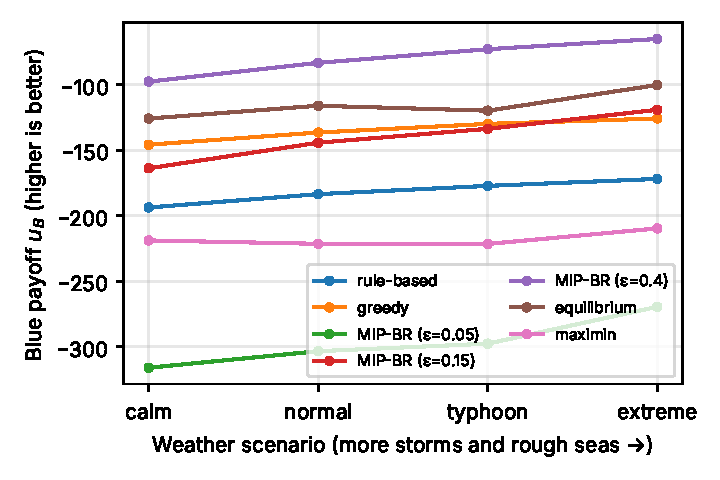
\includegraphics[width=\textwidth]{figures/weather.pdf}
\end{minipage}\hfill
\begin{minipage}{0.63\textwidth}\centering\small
\setlength{\tabcolsep}{3pt}
\begin{tabular}{@{}lrrrrrr@{}}\toprule
Design & Calm & Nom. & Typh. & Extr. & Exp. & Worst\\\midrule
D0 & $-164$ & $-144$ & $-134$ & $-119$ & $-144$ & $-164$\\
D1 & $-153$ & $-141$ & $-131$ & $\mathbf{-98}$ & $-137$ & $-153$\\
D2 & $-181$ & $-164$ & $-149$ & $-136$ & $-162$ & $-181$\\
D3 & $\mathbf{-140}$ & $\mathbf{-118}$ & $\mathbf{-111}$ & $-102$ & $\mathbf{-120}$ & $\mathbf{-140}$\\\bottomrule
\end{tabular}
\end{minipage}
\caption{Left: Blue policy payoffs by weather. Right: Blue design payoffs with MIP-BR on both sides
(reported s.e.\ approximately 7); D0 baseline, D1 basing, D2 sensing, D3 hotline.}\label{fig:rq3}
\end{figure}
\textbf{Weather.} Most tested policies do worst in calm seas: rough seas weaken Red's CCG hulls and storms
pause incidents. Baseline MIP-BR's war rate falls from $0.24$ (calm) to $0.10$ (extreme). MIP-BR with
$\varepsilon_\B=0.40$ and the equilibrium-derived policy rank first and second in all four scenarios.
The highest-payoff policy also has war rates of $0.12$--$0.29$, making sensitivity to $W=200$ important.

\textbf{Designs.} D3 has the best expected and worst-scenario payoff; in nominal weather it cuts war rate
from $0.20$ to $0.05$ and increases Red's payoff from $101$ to $144$. Its zero cost is an assumption.
D1 barely changes Blue's nominal payoff, reduces Red's from $101$ to $16$, and raises war rate to $0.28$.
D2 shows no measurable benefit even in the reported zero-cost check. Red recomputes actions under its
fixed MIP-BR policy; these experiments do not re-solve equilibrium policy selection after redesign.

\textbf{Limits of inference.} Numerical values are assumptions. The findings are comparisons within the model,
not calibrated forecasts of conflict. War rates depend on hazards, de-escalation and war penalties.
Small payoff gaps should be treated cautiously given Monte Carlo error; formal comparisons require
uncertainty estimates for payoff differences. The engine's return-move cap can also make executed positions
differ from the MIP's prescribed fixed positions when returns alone exceed the cap.
